\documentclass[a4paper,11pt]{article}

\usepackage[francais]{babel}
\usepackage[utf8]{inputenc}
\usepackage[pdftex]{graphicx}
\usepackage{hyperref}
\usepackage{color}
\usepackage{fancyheadings}
\usepackage{lastpage}
\usepackage{fullpage}

\newcommand{\HRule}{\rule{\linewidth}{0.5mm}}
\newcommand{\reporttitle}{Attaques timings contre les caches des CPU} % titre en français
\newcommand{\reportauthor}{Jean BAUDINAT, Chloé MACUR}
\newcommand{\reportdate}{\today}

\lhead{}
\rhead{\leftmark \rightmark}
\cfoot{Page \thepage/\pageref{LastPage}}


\begin{document}	
\begin{flushright}
\reportauthor
\end{flushright} 
\vspace{-0.6cm}
\HRule
\begin{center}
{\LARGE \bfseries \reporttitle}
\end{center}

L'utilisation des caches des CPU modifie le temps d'accès à une donnée selon si elle est présente dans le cache ou non. Un attaquant peut alors en tirer des informations et ainsi réaliser une attaque par canal auxiliaire.

\section{Fonctionnement du cache}

Le but du cache est d'accélérer les calculs du processeurs en outrepassant les facteurs limitants que sont la vitesse d'accès à la mémoire ainsi que la bande passante du bus. Au lieu d'accéder à la mémoire via des \emph{load/store}, on accède à une copie des données située dans une mémoire rapide. Lorsque les données auxquelles on souhaite accéder sont présentes dans le cache, on y accède directement sans accès mémoire, on parle alors de \emph{cache hit}. Dans le cas d'un \emph{cache miss} (donnée absente du cache) on va donc accéder à la mémoire et mettre à jour le cache.
  
\begin{figure}[h]
  \centering
  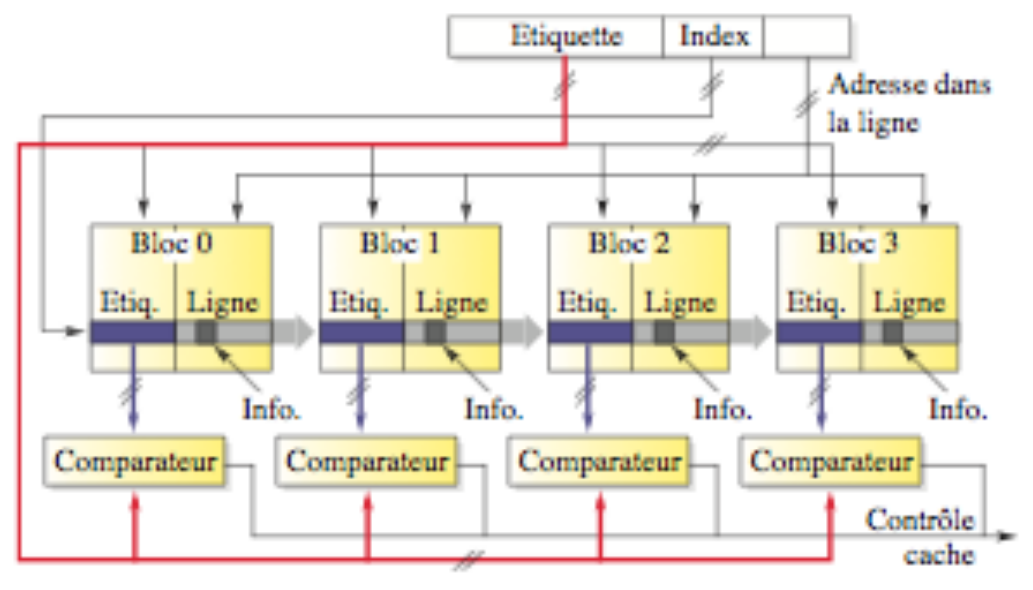
\includegraphics[width=7.5cm]{figures/cache_associative.png}
  \caption{Caches associatifs par blocs (\emph{4-way set associative})}
  \label{cache} 
\end{figure}

Comme présenté dans la figure \ref{cache}, un cache associatif par blocs est constitué de blocs qui contiennent des lignes. Pour identifier une adresse dans le cache on a donc besoin: d'un index (numéro de ligne à tester), de l'adresse dans la ligne (offset du contenu) et d'une étiquette que l'on va comparer avec le contenu de la ligne. On récupère ainsi la valeur désirée dans le cache. 

Lorsqu'un \emph{cache miss} a lieu et que l'on ajoute un contenu dans le cache, s'il n'existe pas de ligne vide on supprime entièrement celle qui a été utilisée le moins récemment (\emph{Least Recently Used, LRU}). On ne récupère pas uniquement les données demandées, mais un mot de taille fixe qui contient les données adjacentes. On notera ainsi qu'en fonction des paramètres du cache (nombre et taille des blocs, taille des mots) et de l'état initial de celui-ci, les données stockées en cache seront différentes.

Le principe du cache étant d'accélérer l'accès aux données, l'accès à la mémoire ne se fait pas en temps constant\footnote{Sur un processeur de 2010, un accès au cache L1 se fait en 0.3ns contre 50 à 150ns pour la mémoire principale~\cite{tromer2010efficient}.}. L'utilisation du cache va donc à la fois modifier la latence et la consommation électrique, permettant à un attaquant d'en déduire l'existence de \emph{cache hit} ou de \emph{cache miss} et ainsi repérer des patterns d'accès à la mémoire et apprendre des informations sur le chiffrement.

\section{Fonctionnement de l'attaque : l'exemple d'AES}

\paragraph{Vulnérabilité d'AES}~\\
Nous allons illustrer la \emph{Cache Timing Attack} en expliquant comment ce type d'attaque peut être mis en œuvre pour casser une implémentation logicielle d'AES\footnote{En effet, l'attaque d'AES est l'exemple le plus référencé dans la littérature de ce type d'attaque.}.

L'attaque d'AES par \emph{Cache Timing Attack} repose sur le stockage en dur des boîtes S dans la mémoire. Ces boîtes S sont utilisées dans l'opération \emph{SubByte} et sont une permutation linéaire de $ GF(256) = GF(2)[x]/(x^8+x^4+x^3+x+1) $ dans lui même. En effet, pour accélérer les calculs, ces boîtes S ne sont pas recalculées en permanence. Elles sont donc stockées en mémoire dans des \emph{Lookup Tables}, et leur utilisation implique leur stockage dans le cache. Les \emph{Lookup Tables} correspondent aux valeurs des boîtes S correspondant à certaines valeurs de clé. Ainsi, l'algorithme peut gagner en rapidité en évitant de charger dans le cache l'intégralité des boîtes S, alors que seule une partie sera utilisée lors du chiffrement. Cependant ces \emph{Lookup Tables} dépendant de la clé, y accéder donne de l'information à l'attaquant et lui permet d'exclure certaines valeurs de clé ne nécessitant pas d'accéder aux \emph{Lookup Tables} chargées en mémoire.

\paragraph{Types d'attaques}~\\
Les \emph{Timing Cache Attack} sont donc des attaques de type canal auxiliaire se basant sur la mesure du temps d'accès à une donnée, selon qu'elle a déjà été stockée dans le cache ou non. Pour être mises en places, ces attaques supposent que la phase de chiffrement est clairement identifiée. On suppose donc que l'adversaire est en mesure d'identifier un changement de contexte, et donc de ne pas utiliser les mesures touchées par ce phénomène. En effet, tout changement de contexte sur le processeur ou se déroule le calcul cryptographique va corrompre le cache, et donc la mesure du temps d'accès.
On suppose de plus que le cache est assez grand pour contenir toutes les informations nécessaires au chiffrement, ce qui est le cas de la plupart des processeurs récents.

On peut alors se donner 3 modèles d'attaquant\cite{aciiccmez2006trace}, selon les informations auxquelles l'attaquant a accès.
L'attaque basée sur le temps (\emph{time driven attack}) repose sur la mesure agrégée du temps de chiffrement. Connaissant la plateforme de chiffrement, l'attaquant est alors en mesure de savoir le nombre de \emph{hit} et de \emph{miss} ayant eu lieu lors de l'opération de chiffrement.
L'attaque basée sur les traces \emph{Trace Driven Attack} est plus précise. L'attaquant peut savoir quand un \emph{hit} ou un \emph{miss} ont lieu. Ce type d'attaque permet donc d'affiner les prédictions sur le type de \emph{Lookup Tables} utilisées.
Enfin, l'attaque basée sur l'accès \emph{Access Driven Attack} suppose que l'attaquant connaît précisément les \emph{lookup tables} auxquelles l'attaquant a pu avoir accès.
Selon le modèle d'attaquant, on voit donc que pour se prémunir face à une \emph{Cache Timing Attack}, le fondeur devra utiliser des méthodes plus ou moins perfectionnées.

\section{Mise en place concrète de l'attaque}

La réalisation de ces attaques contre les caches présente en réalité un certain nombre de difficultés pour l'attaquant. Ainsi, les résultats obtenus lors de l'attaque dépendent évidemment de l'architecture considérée, mais également de l'état initial du cache et de la séquence d'accès à la mémoire. 

\paragraph{État initial du cache} ~\\ 
Il est primordial pour l'attaquant de se placer dans des conditions telles qu'il connaisse l'état initial du cache. Il existe principalement trois états initiaux auxquels il peut se ramener~\cite{canteaut2006understanding}:
\begin{itemize}
\item le cache ne contient pas de tables utiles pour le chiffrement (cache flush, par exemple en coupant l'alimentation)
\item le cache est rempli par l'attaquant (nécessite un accès au cache et donc un système multi-utilisateurs) 
\item le cache contient déjà toutes les tables nécessaires au chiffrement. Cette solution devrait permettre un accès en temps constant à toutes les données, rendant l'attaque difficile. En réalité il subsiste des variations de latence lors de l'exécution de l'algorithme, principalement à cause des conflits dus à des accès concurrents. Par ailleurs, la taille du cache, son architecture ou encore la politique de remplacement peuvent donner lieu à l'éviction de certaines données, et ainsi recréer des \emph{cache miss}.
\end{itemize}

\paragraph{Attaques synchrones et asynchrones} ~\\
On distingue deux types d'attaques selon ce que l'attaquant connaît~\cite{osvik2006cache}. Les attaques dites synchrones supposent que celui-ci peut attaquer en même temps que le chiffrement à lieu et sur le même processeur, lui permettant de connaître des textes clairs. Par exemple un \emph{VPN} (\emph{Virtual Private Network}) peut autoriser un utilisateur lambda à envoyer des paquets. L'attaquant envoie alors des demandes de chiffrement forgées de toutes pièces, lui permettant d'obtenir des informations sur la clé. 

Si jamais l'attaquant ne peut pas communiquer avec le processus de chiffrement et donc ne peut pas l'utiliser à clair connu, il peut tout de même réaliser une attaque dite asynchrone. Ce type d'attaque nécessite une bonne connaissance de l'architecture considérée, mais permet d'obtenir de très bons résultats, notamment dans les processeurs utilisant le \emph{multithreading}. Les prérequis sont alors de pouvoir exécuter un programme sur le même processeur (sans interaction nécessaire entre le processus de l'attaquant et celui de chiffrement), et que la distribution des textes clairs et chiffrés soit non uniforme. En analysant ses propres accès à la mémoire, l'attaquant peut alors identifier des patterns d'accès à la mémoire réalisés par les autres processus. En effet l'introduction de données dans le cache de la part du processus de chiffrement peut évincer des données de l'attaquant, créant ainsi des \emph{cache miss}. Ces statistiques sur l'utilisation des sets de cache sont ensuite comparées avec celles d'AES sur le type de données supposé, et permettent de récupérer des bits de clé. 

\paragraph{Mesure du temps} ~\\
Une difficulté primordiale de cette méthode est de pouvoir mesurer le temps d'accès aux données. Une première méthode~\cite{osvik2006cache} consiste à modifier l'état du cache avant chaque chiffrement. Dans un premier temps on réalise un chiffrement d'un texte clair, ce qui permet de s'assurer que les données désirées sont dans le cache. Puis on les évince du cache en accédant à d'autres données en mémoire, avec une associativité telle que ces nouvelles données remplacent le contenu précédent du cache. On réalise ensuite un second chiffrement du même texte clair et on mesure le temps pris. Selon si les données doivent être remises dans le cache ou non, on mesure un temps différent, et on a donc accès à la différence de temps entre un \emph{cache hit} et un \emph{cache miss}.

Une autre mesure consiste à regarder l'état du cache après l'étape de chiffrement. Pour ce faire l'attaquant remplit d'abord le cache avec des données connues, puis déclenche le chiffrement d'un texte clair, ce qui va évincer une partie des données du cache. Il va ensuite lire toutes les adresses mémoires qu'il avait mises dans le cache et mesurer le temps que ça prend. Si le processus de chiffrement n'a pas accédé à certains sets de cache, l'accès donnera lieu à un \emph{cache hit}, et on aura un \emph{cache miss} dans le cas contraire, ce qui donne bien une différence lors de la mesure du temps. L'avantage de cette méthode par rapport à la précédente est qu'elle permet de mesurer tout à la fin et en un seul coup, elle est donc beaucoup moins sujette à des variations de temps et donc plus précise.

\section{Contre-mesures}

L'évolution des technologies matérielles ainsi que les contre-mesures rendent la \emph{Timing Cache Attack} plus difficile à mettre en \oe uvre.

\paragraph{Une attaque sur x86 plus difficile}~\\
Mowery~\cite{mowery2012aes} cite des évolutions matérielles rendant plus difficile voir impossible la mise en œuvre de l'attaque d'AES. Parmi celles-ci, on compte notamment le nouveau jeu d'instruction des processeurs Intel : AES-NI. Ce jeu d'instruction permet de traiter matériellement sur un composant dédié du processeur le chiffrement AES. Ainsi, il n'est plus du tout fait usage du cache. Le clair est chargé, et le chiffré est calculé sans aucune autre interaction avec la mémoire ou le cache. Cette innovation a été suivie par d'autres fondeurs. Un processeur possédant ce type de composant sera donc virtuellement à l'abri de ce type d'attaque. Cependant, encore faut-il que l'implémentation d'AES utilise le bon jeu d'instructions, ce qui n'est pas toujours le cas.

\paragraph{Une évolution des technologies créatrice de difficultés supplémentaires}~\\
\begin{figure}[h]
  \centering
  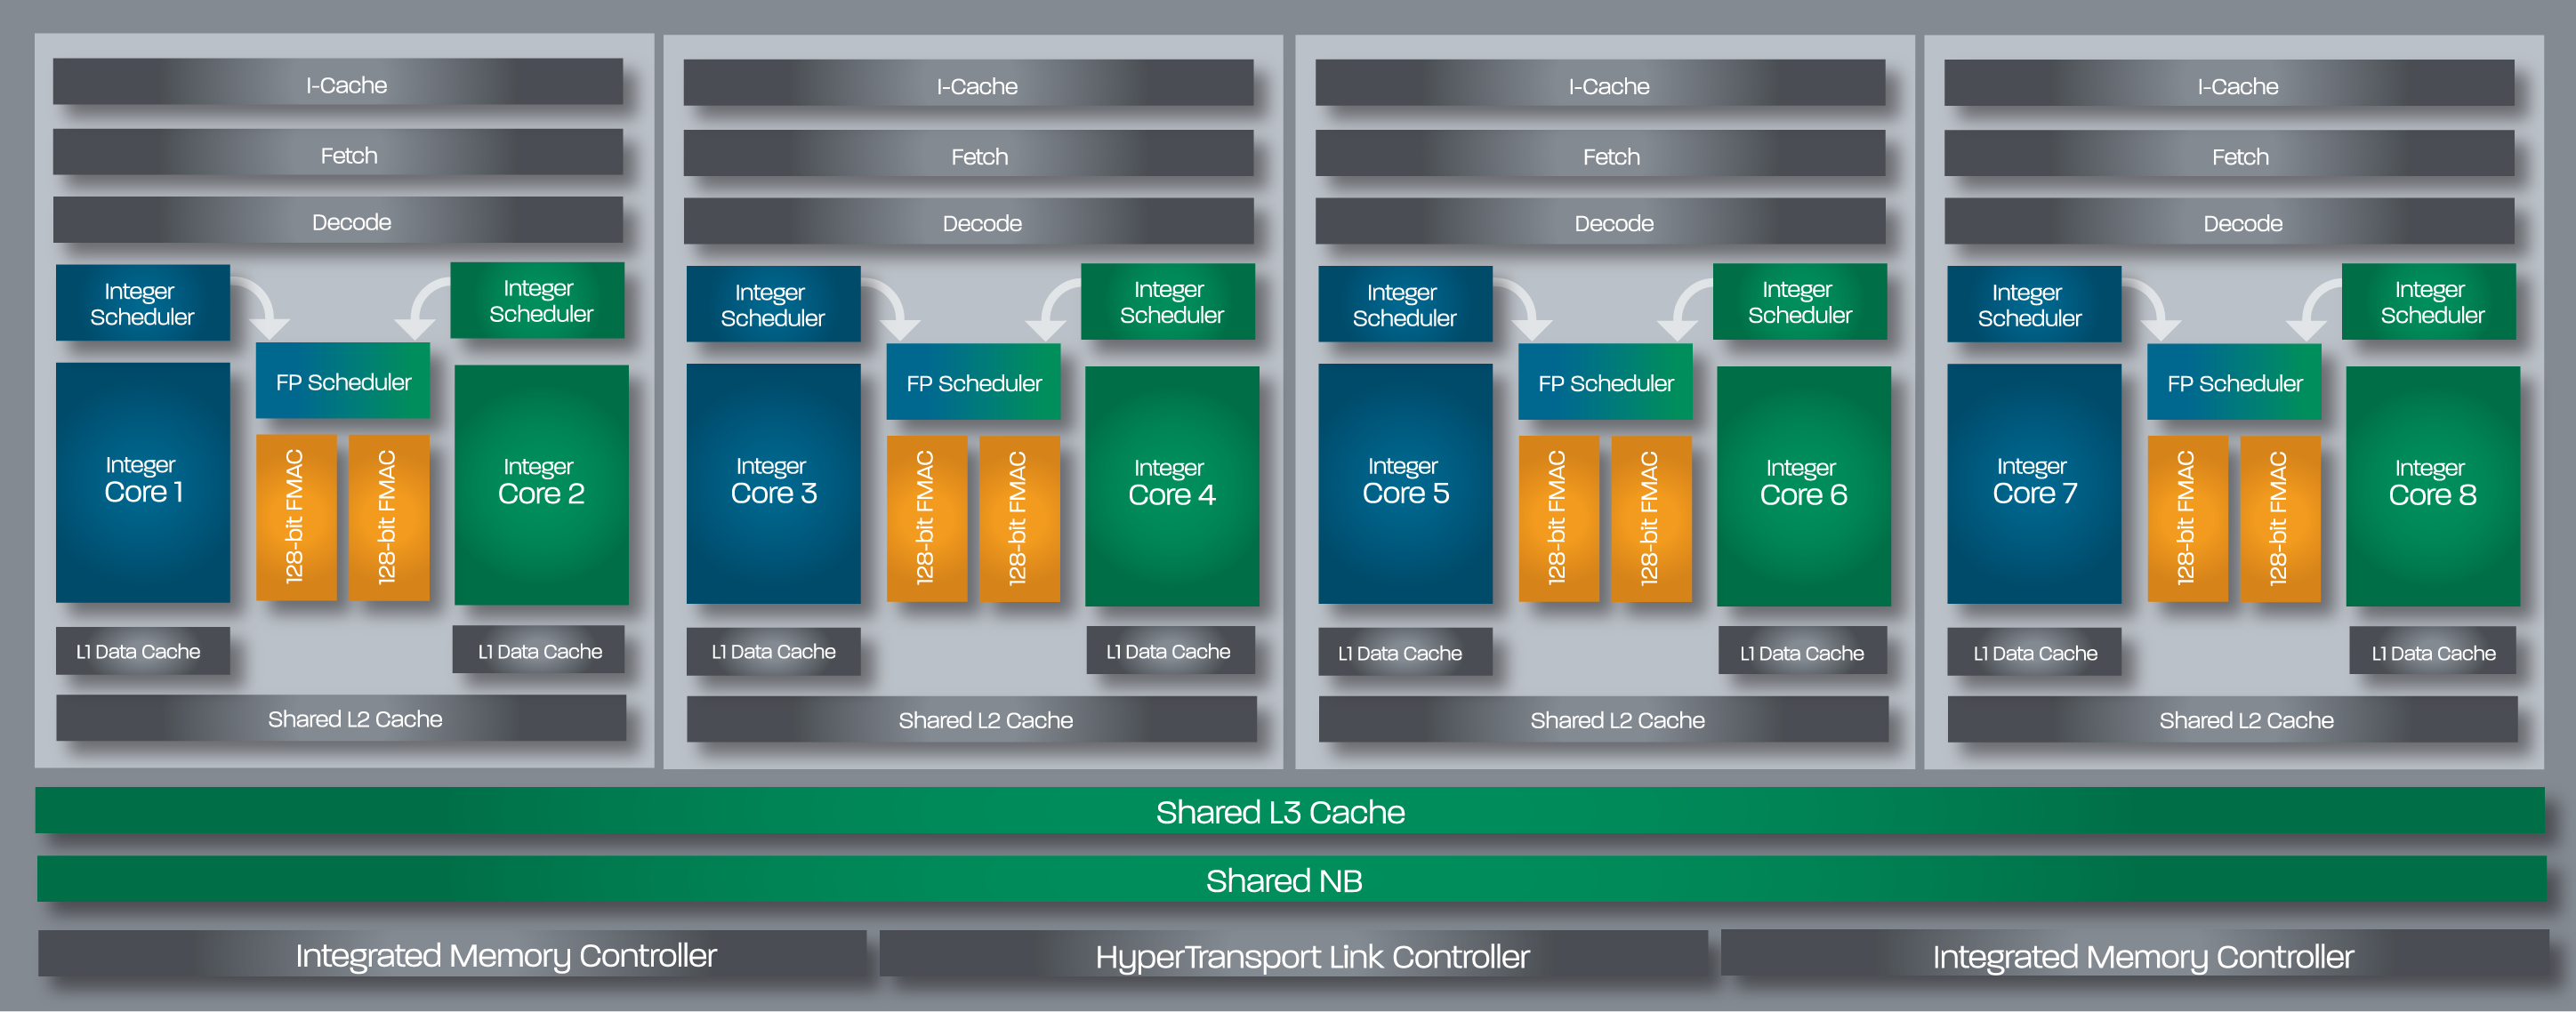
\includegraphics[width=13cm]{figures/BDArch.png}
  \caption{Étagement des caches dans un processeur quadricoeur}
  \label{etagement} 
\end{figure}
L'évolution des technologies actuelles a entraîné l'apparition de deux phénomènes. Tout d'abord, les processeurs sont désormais multicœurs, ce qui leur permet de faire tourner plusieurs processus en même temps. Cette évolution, destinée à accélérer le traitement des données a également des répercussion sur la mise en place de la \emph{Cache Timing Attack}\cite{weiss2012cache}. Dans le cas du processeur quadricœur d'Intel  présenté sur la Figure \ref{etagement} par exemple, chaque cœur possède deux \emph{threads} possédant chacun leur cache L3. Le cœur lui même possède son cache L2. Enfin, l'ensemble du processeur possède un cache L1. Cette multiplication des caches en étage complexifie l'attaque puisqu'elle occasionne plus de bruit lors de la mesure des \emph{hit} ou \emph{miss} intéressants, les caches L3 et L2 étant corrompus par les processus tournant sur les autres cœurs et \emph{threads}.

Une autre évolution réside dans la virtualisation des tâches, tendant à séparer les processus et les contextes. \cite{weiss2012cache}. 
%TODO  reformuler, pas compréhensible. Pourquoi "cependant"? "dans ces cas"?
Cependant, l'attaque exploitant les caches est dans ces cas une des seules qui puisse être mise en oeuvre depuis un environnement non sécurisé vers un environnement sécurisé.
C'est par exemple le cas sur les environnement de type téléphone mobile, où l'OS et l'environnement sécurisé effectuant les opérations de cryptographie sont séparés par de la virtualisation. Cependant, un attaquant corrompant l'OS (à l'aide d'un cheval de Troie par exemple) pourra par la suite mener une \emph{Cache Timing Attack} contre l'environnement sécurisé, le cache étant partagé malgré la virtualisation.

\paragraph{Implémentation d'un algorithme en temps constant: le cas d'AES} ~\\
Puisque la mesure du temps d'accès aux données permet d'obtenir des informations sur la clé de chiffrement, une solution pour pallier à cette exploitation serait d'implémenter un algorithme AES en temps constant\footnote{"En temps constant" signifie indépendant de la clé AES et du texte clair.}. Il est possible d'écrire de tels algorithmes qui n'utilisent pas les boîtes~S\footnote{On pourrait également ajouter une boucle de durée d'exécution connue qui tourne jusqu'à atteindre le pire temps d'exécution connu.} mais le temps d'exécution est beaucoup trop élevé.
On souhaiterait alors s'assurer que les boîtes S sont dans le cache pendant toute la durée du chiffrement.

Une solution proposée par Bernstein~\cite{bernstein2005cache} est d'ajouter une instruction aux CPU qui s'assurerait que toutes les tables sont bien dans le cache L1, et qui pourrait charger une table en un nombre constant de cycles. On peut imaginer que l'instruction utilise un bit pour se souvenir que l'ensemble de la table est dans le cache L1, évitant ainsi de vérifier la fois suivante, auquel cas on conserve la rapidité spécifique au cache. Si jamais des registres sont modifiés ou bien une ligne évincée du cache, le bit est réinitialisé, mais le chargement de la table se fait en temps constant quelles que soient les lignes manquantes.

Un autre moyen d'éviter que les variables utilisées lors du chiffrement soient évincées du cache consiste à les mettre côte à côte en mémoire. On peut ainsi positionner la clé AES, le texte clair, le texte chiffré ainsi que les boîtes S de manière adjacente dans le cache L1.

Pour pallier aux interruptions du code, durant lesquelles les boîtes S peuvent sortir du cache, on peut imaginer que le noyau désactive les interruptions lors du chiffrement AES. Une autre solution serait, si une interruption ou un événement anormal a lieu, de volontairement vider le contenu du cache afin d'éviter que toute information soit récupérée~\cite{canteaut2006understanding}.

Par ailleurs, Käsper~\cite{kasper2009faster} présente une implémentation de DES en temps constant qui remplace les instructions conditionnelles par des séquences d'instruction déterministes, afin d'éviter toute fuite d'information. 
Ce papier propose également de désactiver le multithreading afin de rendre l'attaque plus difficile. En allouant un cœur à l'opération de chiffrement, et en interdisant à d'autres processus de s'exécuter, on empêche ainsi les mesures logicielles sur les caches L1 et L2.

Une autre approche~\cite{osvik2006cache} consiste à ajouter du bruit en réalisant en parallèle le chiffrement d'un texte inutile. Il faut noter que cette technique oblige simplement l'attaquant à utiliser davantage d'échantillons, mais ne rend pas l'attaque impossible pour autant. Ce papier évoque également la possibilité de désactiver le cache, ou encore de l'utiliser en mode \emph{no-fill}. 



\section*{Conclusion}
L'utilisation des caches fournit des temps d'accès aux données variables, permettant à un attaquant d'obtenir des informations sur le matériel cryptographique. Un certain nombre de techniques visant à empêcher cette attaque ne font que la rendre plus difficile, et sont grandement dépendantes de l'architecture considérée. Par ailleurs, si l'implémentation d'algorithmes en temps constant permet en théorie d'empêcher l'attaque, ils sont en pratique difficiles à réaliser et conduisent à une baisse de performance.

La seule solution pleinement satisfaisante actuellement permettant de se prémunir face à ce type d'attaque auxiliaire semble donc être l'implémentation d'une puce cryptographique effectuant le calcul, et évitant ainsi l'usage de cache. Cependant, cette solution est coûteuse, et suppose l'usage exclusif de l'algorithme qu'elle supporte. 
Par ailleurs, même en réussissant à se prémunir face à l'usage des caches comme canal auxiliaire, d'autres composants du processeur peuvent avoir une incidence sur la sécurité des algorithmes de chiffrement, comme les composant de branchement prédictif par exemple.

\newpage
\bibliographystyle{unsrt}
\bibliography{ref}


\end{document}
